\documentclass{article}
\usepackage[]{amsmath}
\usepackage[]{hyperref}
\usepackage[]{graphicx}
\usepackage{xcolor}
\usepackage[backend=biber,style=numeric]{biblatex}

\addbibresource{ipe.bib}

\def\Ipe{\textsc{Ipe}}
\title{IpePlots -- User Manual with Examples}
\author{Jan Hlavacek\\(jhlavace@svsu.edu)}
\begin{document}
\maketitle
\tableofcontents
\begin{abstract}
   IpePlots is an extension (so called ``ipelet'') for the graphics editor \Ipe\
   (\url{http://ipe7.sourceforge.net}).  The purpose of this extension is to
   make creation of plots of functions, especially the type of plots used in
   mathematics education, easier.  We provide basic introduction to IpePlots,
   as well as several step by step examples. 
\end{abstract}

\section{Introduction}
The \Ipe\ graphics editor, written by Otfried Cheong, is a drawing editor for
creating figures in PDF or encapsulated PostScript format. According to the Ipe
website\cite{ipeweb}, its main features are:
\begin{itemize}
   \item Entry of text as \LaTeX\ source code. This makes it easy to enter
      mathematical expressions, and to reuse the \LaTeX-macros of the main
      document. In the display text is displayed as it will appear in the
      figure.
   \item Produces pure Postscript/PDF, including the text. \Ipe\ converts the \LaTeX-source to PDF or Postscript when the file is saved.
   \item  It is easy to align objects with respect to each other (for instance,
      to place a point on the intersection of two lines, or to draw a circle
      through three given points) using various snapping modes.
   \item  Users can provide ipelets (\Ipe\ plug-ins) to add functionality to
      \Ipe. This way, \Ipe\ can be extended for each task at hand.
   \item  \Ipe\ can be compiled for Unix and Windows.
   \item  \Ipe\ is written in standard C++ and Lua 5.1. 
\end{itemize}
IpePlots is a plotting extension for the \Ipe. Its can help you include plots
of functions, parametric curves and coordinate systems into your \Ipe\
drawings.  IpePlots is written in Lua 5.1.  It is released under the GPL v.2.0.

\section{Installation}

We will assume that you already have the \Ipe\ graphics editor installed on
your computer.  You can obtain the editor from the \Ipe\ webpage\cite{ipeweb}. 

Installation of IpePlots is very simple.  All you have to do is to place the
file \texttt{plots.lua} in the ``ipelets'' directory on your computer.  On Unix
and Unix-like systems, you can use for example the \verb|$HOME/.ipe/ipelets|
directory.  On Windows, the directory is determined by the value of the
\texttt{IPELETPATH} environment variable.  After installing IpePlots, simply
restart \Ipe.  If the installation was successful, you will have a ``Plots''
sub-menu under \Ipe's ``Ipelets'' menu (Figure~\ref{fig:ipewindow}).
\begin{figure}[h]
   \begin{center}
      %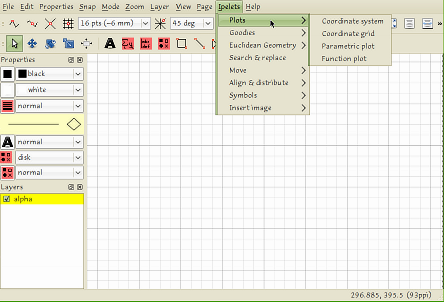
\includegraphics{ipewindow_small.png}
      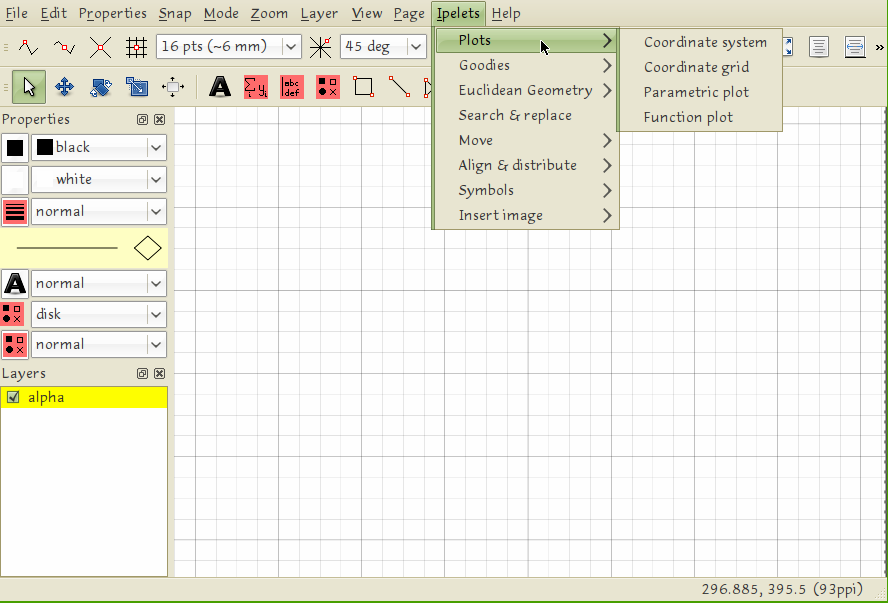
\includegraphics[scale=3]{ipewindow.png}
   \end{center}
   \caption{\Ipe\ window with the ``Plots'' sub-menu open}
   \label{fig:ipewindow}
\end{figure}

\section{Usage}
To insert a plot or a coordinate system into your drawing, select one of the
items in the ``Plots'' sub-menu under the ``Ipelets'' menu.  In the current
version of IpePlots, there are four items:
\begin{description}
   \item[Coordinate system] will insert a Cartesian coordinate system into your
      drawing.  It will consist of the horizontal axis, the vertical axis, and
      optional tics.  IpePlots currently does not create any labels, if you
      want to label the axes or tics, you have to do so manually.
   \item[Coordinate grid] will insert a rectangular grid of vertical and
      horizontal line segments into your drawing.  You can specify the location
      of the segments. 
   \item[Parametrid plot] will insert a parametric curve defined by two
      functions, $x = f(t)$ and $y = g(t)$.
   \item[Function plot] will insert a plot of a function $y = f(x)$. 
\end{description}
Depending of several things, IpePlots will do one of the following:
\begin{itemize}
   \item If your current selection has a non-empty bounding box, IpePlot will
      use this bounding box as a ``viewport'' which will contain the coordinate
      system of the plot.
   \item If you do not have a current selection, or if the selections bounding
      box is empty, IpePlot will use the canvas coordinate system in the
      following way:
      \begin{itemize}
	 \item If you previously set the origin of the \Ipe\ axis system, it
	    will be used as the origin of the plot coordinate system.  The
	    base direction of the axis system is ignored, however, and the plot
	    axis are always created horizontal and vertical. 
	 \item If you did not set the origin of the axis system, the absolute
	    canvas coordinates are used instead. 
      \end{itemize}
\end{itemize}

After selecting one of the menu items, you will be presented with a dialog box. 

The current version of IpePlots provides the following four menu items:

\subsection{Coordinate System}
creates a pair of coordinate axes, with optional ticks. If the current
selection has a non-empty bounding box, the axes will be scaled so that they
will exactly fit inside this bounding box. In the dialog box
(Figure~\ref{fig:coord_sys_dialog}) you can set the range for $x$, the range for
$y$, the optional size of ticks (defaults to 0 for no ticks), and the location
of ticks (if left empty, and the size is non-zero, ticks are placed at integer
coordinates). 

\begin{figure}[h]
   \begin{center}
      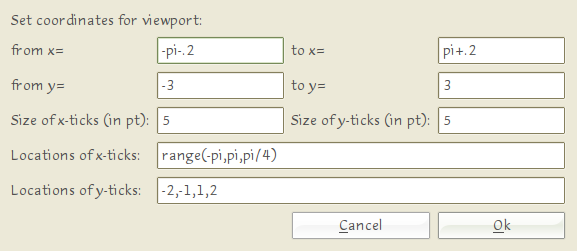
\includegraphics[scale=3]{coord_sys_dialog.png}
   \end{center}
   \caption{Dialog box for the Coordinate System}
   \label{fig:coord_sys_dialog}
\end{figure}

Note that in all fields except the two tick size fields, you can use Lua
expressions, which makes it possible to enter values like \texttt{-pi - 0.2} or
\texttt{sqrt(3)/2}. 

The syntax for the location of ticks is special: you could specify a comma
separated list of numbers, or you could enter a single Lua table containing
numbers.  That way you can enter a Lua expression that generates a table of
numbers.  For example, IpePlots provides an internal function
\texttt{range(from, to, step)} which produces a table of numbers starting with
the value of ``\texttt{from}'' and incrementing by ``\texttt{step}'' until it
exceeds ``\texttt{to}''.  The values entered in the
Figure~\ref{fig:coord_sys_dialog} will produced the coordinate system in
Figure~\ref{fig:coord_sys}. Note that the rectangle containing the coordinate
system was not created by IpePlots.  It was already present in the drawing, and
we selected it before using IpePlots.  The coordinate system was created by
IpePlots in such a way that it fits perfectly inside the bounding box of the
rectangle. The rectangle can be deleted after the coordinate system is created. 

\begin{figure}[h]
   \begin{center}
      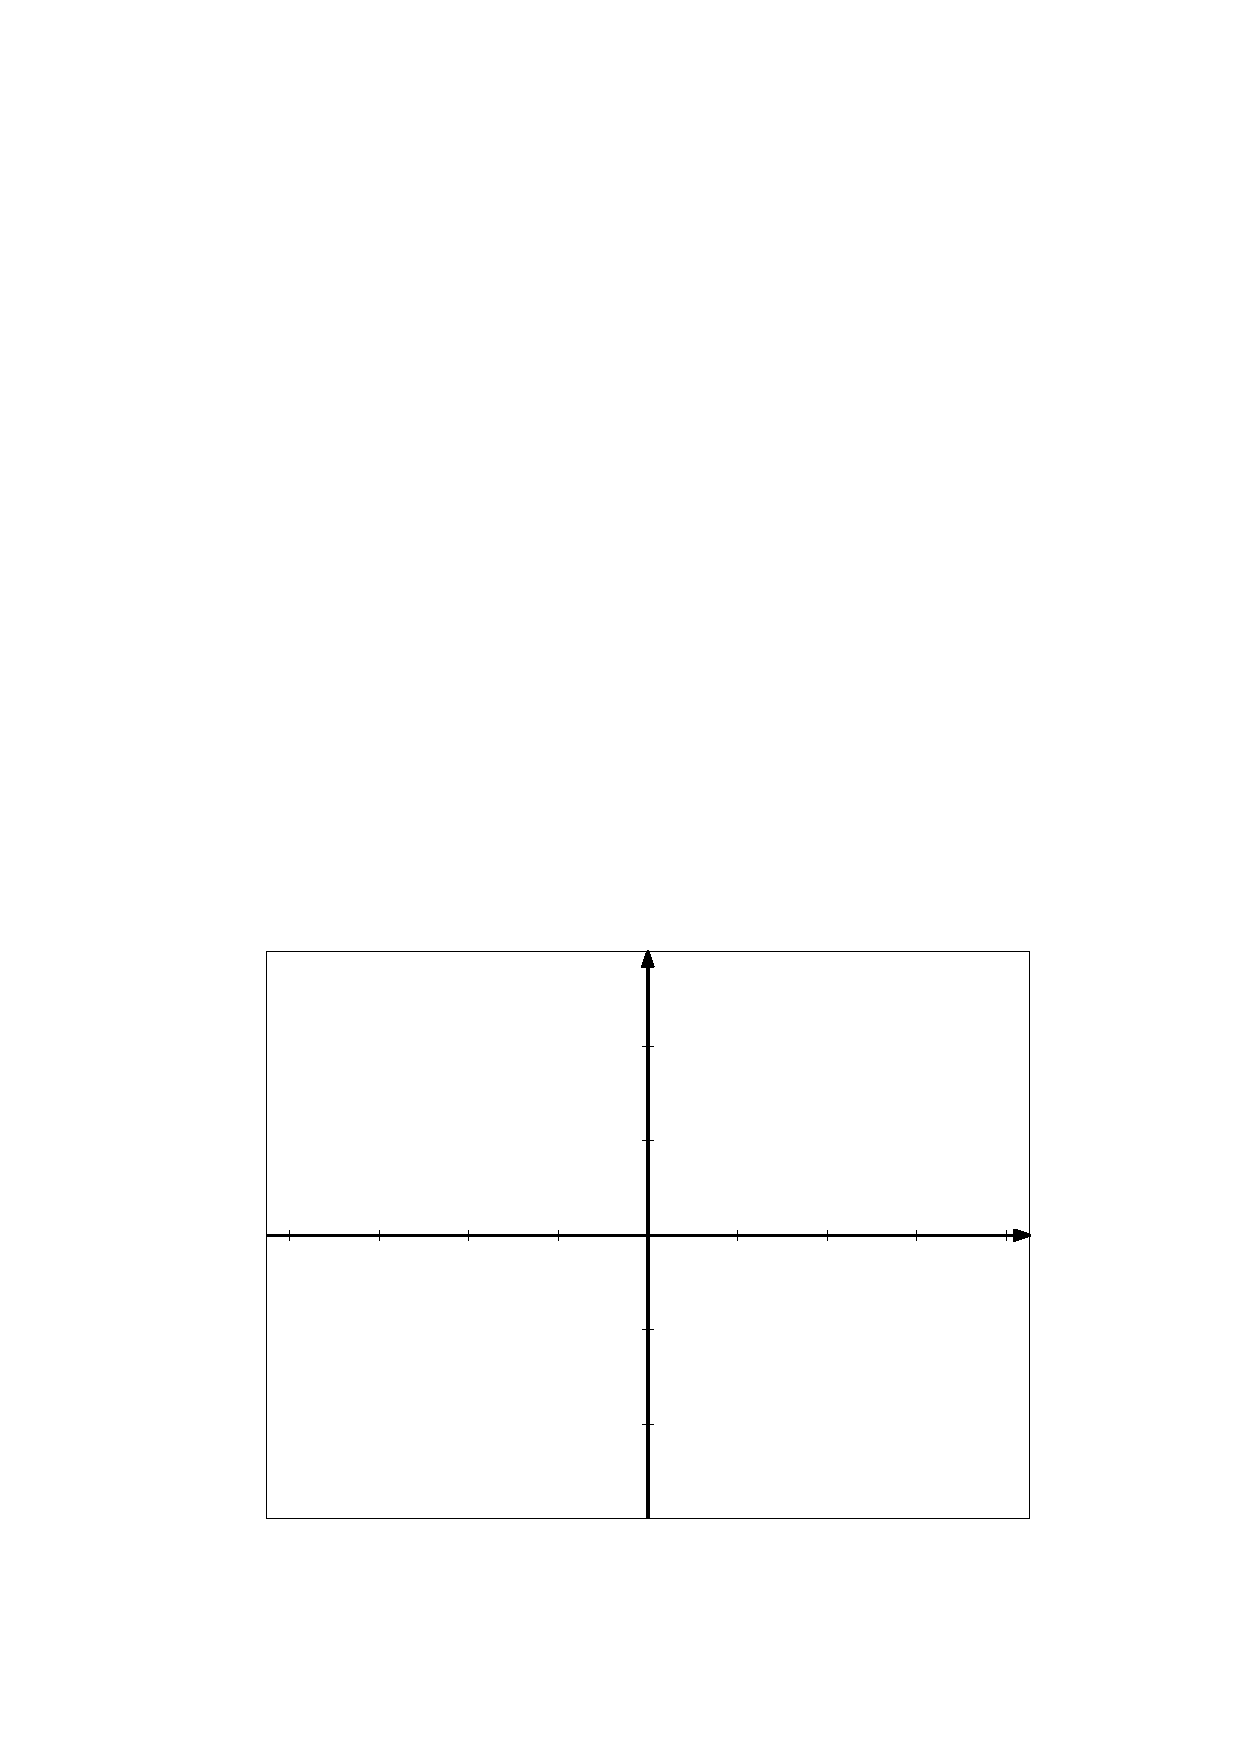
\includegraphics[scale=.7]{coord_sys}
   \end{center}
   \caption{An example of a coordinate system produced by IpePlots.}
   \label{fig:coord_sys}
\end{figure}

Also note that IpePlots does not create labels.  We see that as an advantage.
IpePlots will quickly create a axes system for you, and you can then label it
in any way you want, IpePlots will not impose any labeling style on you. \Ipe's
vertex snapping mode  and the ``align'' and ``move'' ipelet groups can be very
helpful when adding labels. 

If your selection is empty, or has an empty bounding box, you will be presented
with the same dialog box, however, instead of scaling the coordinates in order
to fit them into the given bounding box, IpePlots will use the absolute canvas
coordinates.  That means a coordinate system from $-\pi$ to $\pi$ would be
really small, so it is probably more useful to specify coordinates like $-50$
to $50$. 

\subsection{Coordinate Grid}
will create a rectangular grid of horizontal and vertical line segments at
specified coordinates. The dialog box (see Figure~\ref{fig:coord_grid_dialog}) is
very similar to the dialog box for Coordinate System, except that there are no
fields for tick size, and instead of tick locations, you specify the locations
of vertical and horizontal grid lines. 

\begin{figure}[h]
   \begin{center}
      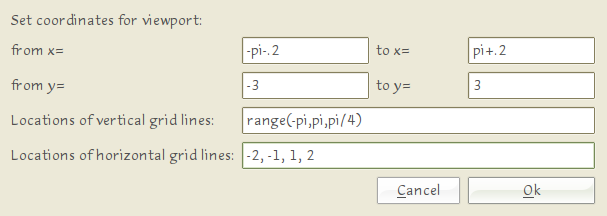
\includegraphics[scale=3]{coord_grid_dialog.png}
   \end{center}
   \caption{Dialog box for the Coordinate System}
   \label{fig:coord_grid_dialog}
\end{figure}

The coordinate grid created by IpePlots with the values filled in as in
Figure~\ref{fig:coord_grid_dialog} will produce the coordinate grid in
Figure~\ref{fig:coord_grid}.  Again, the rectangle containing the coordinate
grid was not created by IpePlots.  IpePlots created the coordinate grid inside
the existing rectangle. 

\begin{figure}[h]
   \begin{center}
      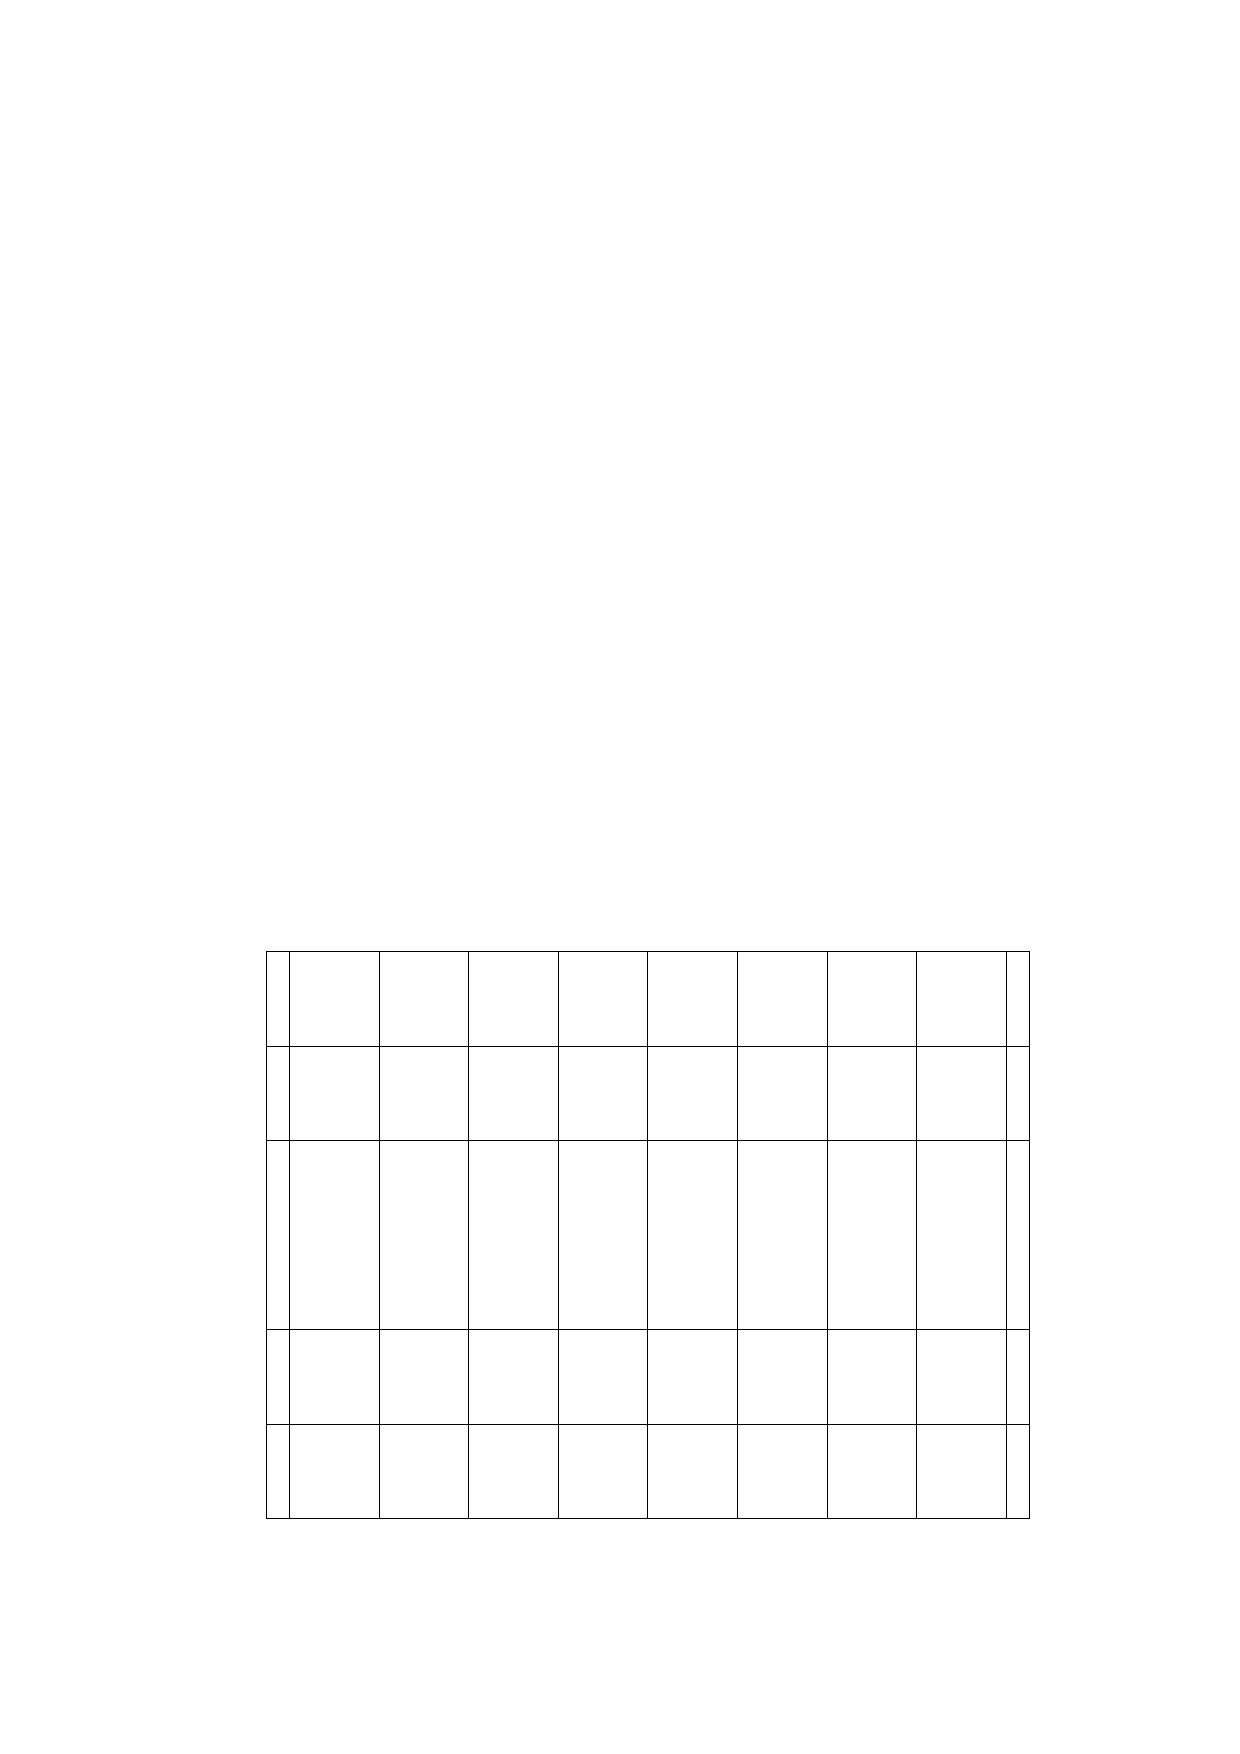
\includegraphics[scale=.7]{coord_grid}
   \end{center}
   \caption{An example of a coordinate grid produced by IpePlots.}
   \label{fig:coord_grid}
\end{figure}

Note that only the coordinate grid was created, not the coordinate axes.  If
you want to create both, you have to use both ``Coordinate System'' and
``Coordiate Grid'' items from the ``Plots'' menu.  You can find some examples
of a complete work flow in section~\ref{sec:examples} on
page~\pageref{sec:examples}. 

As for Coordinate System, if the current selection is empty or has an empty
bounding box, IpePlot will use the absolute canvas coordinates when creating
the grid. 

\subsection{Parametric Plot}
creates a plot of a curve described by the parametric equations
\begin{align*}
   x &= f(t)\\
   y &= g(t)\\
   a &\le t \le b
\end{align*}
The dialog box for Parametric Plot is shown in the
Figure~\ref{fig:param_dialog}. You need to specify $x$ and $y$ as functions of
a parameter $t$, and the bounds for $t$. If the current selection has a
non-empty bounding box, you also have to specify the ranges of $x$ and $y$
coordinates that correspond to the bounding box.  The plot will be scaled in
such a way that the given $x$ and $y$ coordinate ranges will fit exactly into
the bounding box. 

\begin{figure}[h]
   \begin{center}
      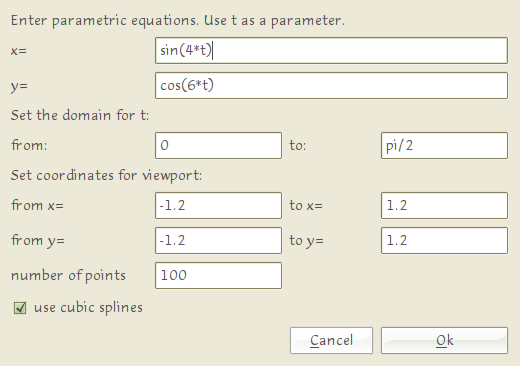
\includegraphics[scale=3]{param_dialog.png}
   \end{center}
   \caption{Dialog box for the Parametric Plot}
   \label{fig:param_dialog}
\end{figure}

You also need to specify the number of points used to draw the plot.  The more
points you use, the more precise is your plot going to be.  On the other hand,
the more points you specify, the larger the file containing the drawing, and
with large number of points, \Ipe\ may slow down significantly, especially on
systems with low resources. The default of $100$ seems to generally be a
reasonable compromise.

Finally, you can select whether you want the plot to be approximated by cubic
splines or by series of line segments. Cubic splines will generally produce a
smoother curve.  Note that if you have less than 4 points specified, the cubic
spline option will be ignored. 

The plot generated from the values entered in Figure~\ref{fig:param_dialog} is
shown in Figure~\ref{fig:param}.  Again, the rectangle containing the Lissajous
curve was not generated by IpePlots. It was used as a bounding box, which will
exactly represent the coordinate rectangle $-1.2\le x \le 1.2$, $-1.2\le y \le
1.2$. 

\begin{figure}[h]
   \begin{center}
      
\includegraphics[scale=.7]{param}
   \end{center}
   \caption{An example of a parametric plot produced by IpePlots.}
   \label{fig:param}
\end{figure}

If the current selection is empty or has an empty bounding box, there is no
need to specify the ranges of $x$ and $y$ coordinates, since IpePlots will be
using the absolute canvas coordinates.  The dialog box presented to you in such
a case will not have the fields for these coordinates.  You can use this mode
to insert precise curves in the absolute canvas coordinates into your drawing.
For example, the ornamental curve in Figure~\ref{fig:spliced_curve} was created by
combining a partial Lissajous curve in absolute canvas coordinates with two
semicircles.

\begin{figure}[h]
   \begin{center}
      
\includegraphics[scale=.5]{spliced_curve}
   \end{center}
   \caption{An example of a curve created by combining a parametric curve in
   absolute canvas coordinates with two semicircles.}
   \label{fig:spliced_curve}
\end{figure}

\subsection{Function Plot}
creates a graph of a function $y = f(x)$. Note that IpePlots has no special
treatment for things like discontinuities, asymptotes etc. See the
section~\ref{subsec:asymptote} on page \pageref{subsec:asymptote} to see an
example of plotting a graph of a function with a vertical asymptote.

\begin{figure}[h]
   \begin{center}
      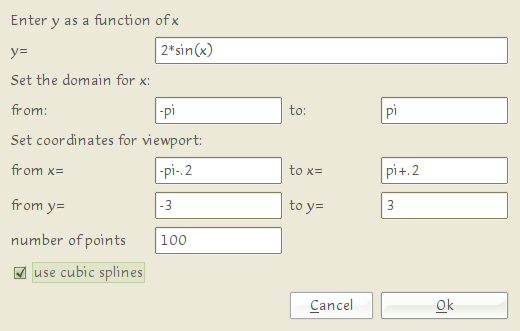
\includegraphics[scale=3]{function_dialog.png}
   \end{center}
   \caption{Dialog box for the Function Plot}
   \label{fig:function_dialog}
\end{figure}

The dialog box for the Function Plot is shown in
Figure~\ref{fig:function_dialog}.  In this dialog, you need to enter the actual
function, the domain over which the function should be graphed, and the
coordinate limits for the bounding box. If the current selection is empty or
has an empty bounding box, the limits for the bounding box will not be present
in the dialog.  Just as in the parametric plot dialog, you can change the
number of points used to draw the graph, and choose whether you want to use
line segments or cubic splines to approximate the curve. 

\begin{figure}[h]
   \begin{center}
      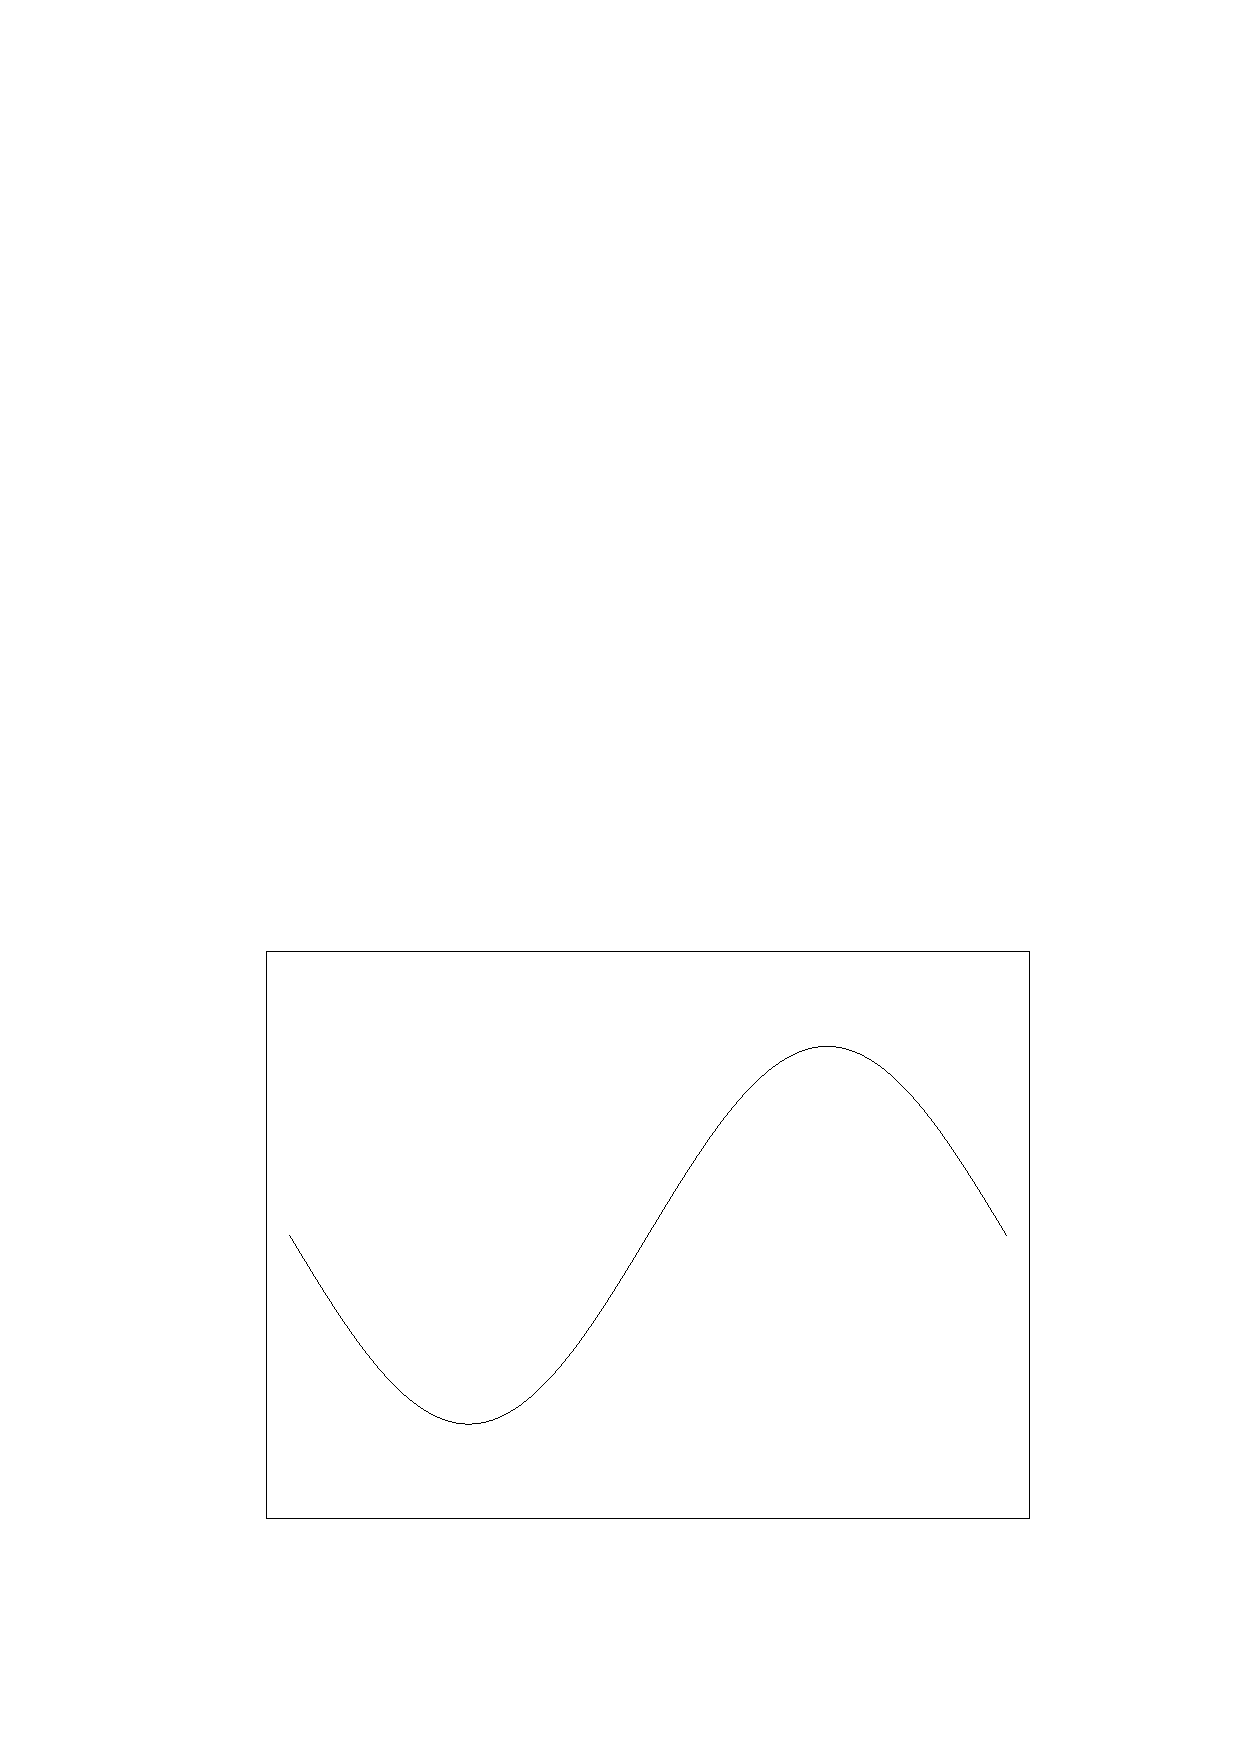
\includegraphics[scale=.5]{function}
   \end{center}
   \caption{An example of a graph of a function produced by IpePlots.}
   \label{fig:function}
\end{figure}

The graph created from the parameters entered in
Figure~\ref{fig:function_dialog} is shown in Figure~\ref{fig:function}. As
before, the rectangle containing the graph was not created by IpePlots,
instead it was used as a bounding box to fit the graph into. 

\clearpage
\section{Examples}\label{sec:examples}
\subsection{Plotting a Piecewise Function}
In this example we will create a plot of the piecewise defined function:
\[
f(x) = 
\begin{cases}
   x + 5 & \text{ if $x <= -2$}\\
   x^2 - 1 & \text{ if $-2 \le x < 1$}\\
   2 - x & \text{ if $x \ge 1$}
\end{cases}
\]

To show all the features, we will create a viewing rectangle approximately $-5
< x < 5$ and $-4 < y < 4$. 

In order to create a plot with a $1:1$ aspect ratio, we need start by creating
a rectangle with the ratio of horizontal to vertical side $5:4$.  We can
conveniently use the grid snapping mode in \Ipe (see the \Ipe\
manual(\cite{manual}) for details).  An example of such rectangle
is shown in the Figure~\ref{fig:piecewise_starting_rectangle}  Notice that the
rectangle is shown in {\color{red}red}, which means that it is currently
selected. 
\begin{figure}[h]
   \begin{center}
      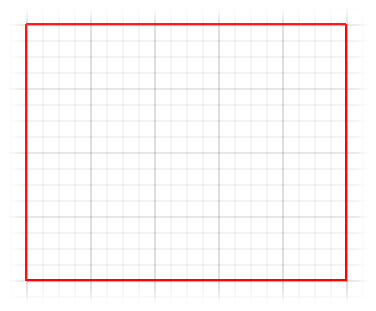
\includegraphics[scale=2]{piecewise_starting_rectangle.png}
   \end{center}
   \caption{A rectangle with $5:4$ side ratio}
   \label{fig:piecewise_starting_rectangle}
\end{figure}

Making sure the rectangle is selected, choose the ``Coordinate System'' entry
from the ``Plots'' menu, and fill in the dialog as shown on
Figure~\ref{fig:piecewise_system_dialog}.  Note that the fields for location of
ticks are left empty, which means that ticks will appear at every integer.  This will define the viewing
rectangle, and create the $x$ and $y$ axes, with 5 pt long ticks at every
integer (Figure~\ref{fig:piecewise_system}).  
\begin{figure}[h]
   \begin{center}
      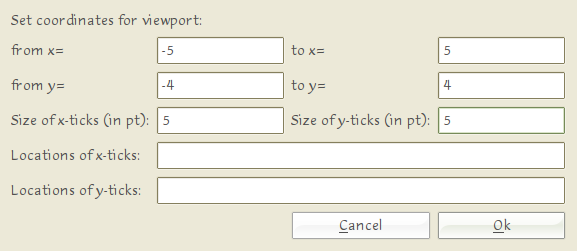
\includegraphics[scale=3]{piecewise_system_dialog.png}
   \end{center}
   \caption{The dialog box for coordinate system}
   \label{fig:piecewise_system_dialog}
\end{figure}

\begin{figure}[h]
   \begin{center}
      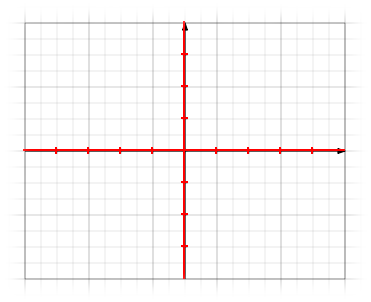
\includegraphics[scale=2]{piecewise_system.png}
   \end{center}
   \caption{The coordinate system created by the dialog box in
   Figure~\ref{fig:piecewise_system_dialog}} 
   \label{fig:piecewise_system}
\end{figure}

After creating the coordinate system, it should be selected.  If it is not,
select it using the ``select'' tool. The next step will be creating a
coordinate grid.  Select the ``Coordinate grid'' entry from the ``Plots'' menu.
The Coordinate grid dialog will appear, with information already filled
(Figure~\ref{fig:piecewise_grid_dialog}).
IpePlots automatically filled in this information based on the data you
entered in the ``Coordinate system'' dialog.  If you are happy with these
choices, you can just click the OK button.  The coordinate system shown in
Figure~\ref{fig:piecewise_grid} will be created. It will be created with the
currently active line style.  For our purpose, we want to change this into
dashed style using the \Ipe\ properties panel. 

\begin{figure}[h]
   \begin{center}
      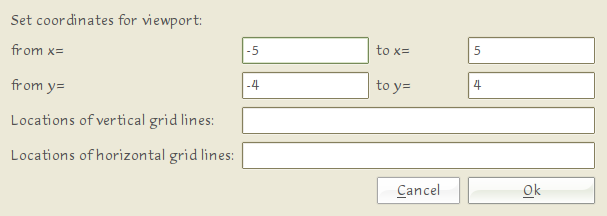
\includegraphics[scale=3]{piecewise_grid_dialog.png}
   \end{center}
   \caption{The dialog for creation of a coordinate grid}
   \label{fig:piecewise_grid_dialog}
\end{figure}

\begin{figure}[h]
   \begin{center}
      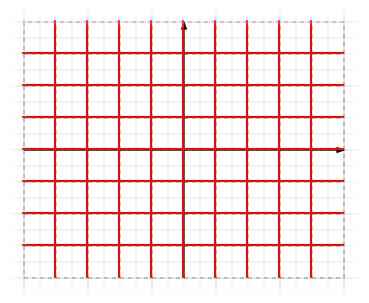
\includegraphics[scale=2]{piecewise_grid.png}
   \end{center}
   \caption{The coordinate grid created by the dialog box in
   Figure~\ref{fig:piecewise_grid_dialog}}
   \label{fig:piecewise_grid}
\end{figure}

Now we need to create the first part of the graph: $y = x+5$ for $x < -2$. Make
sure that either the coordinate system or the coordinate grid is selected.
Then choose ``Function plot'' from the ``Plots'' menu. As before, the dialog is
partially filled based on the information that you entered in the previous
dialogs.  Fill in the remaining entries as shown on
Figure~\ref{fig:firstline_dialog}. Note that since we are plotting a line
segment, we only need to use 2 points, and we do not want to use cubic
splines\footnote{The figure will look perfectly fine with larger number of points, and of
course when using cubic spline to approximate a linear function, we get the
correct linear function, however, it would make IpePlots generate more
complicated code, which would then result in a larger file.}. You can see the result in
Figure~\ref{fig:firstline}.  

\begin{figure}[h]
   \begin{center}
      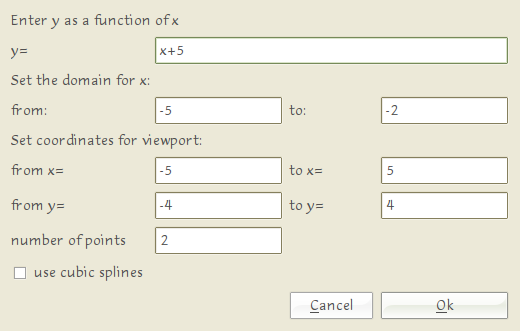
\includegraphics[scale=3]{firstline_dialog.png}
   \end{center}
   \caption{The dialog box that will create the first part of the plot: $y =
   x+5$ for $x < -2$}
   \label{fig:firstline_dialog}
\end{figure}

\begin{figure}[h]
   \begin{center}
      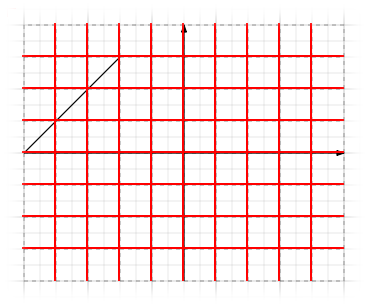
\includegraphics[scale=2]{firstline.png}
   \end{center}
   \caption{The first part of the plot of the piecewise function}
   \label{fig:firstline}
\end{figure}

The next part of the plot is the parabolic arc $y = x^2 - 1$ for $-2 \le x <
1$.  First select either the coordinate system or the coordinate grid in which
the parabola should be placed.  Then choose ``Function plot'' from the
``Plots'' ipelet menu.  The dialog box that will open will contain the values
that you entered when plotting the first part.  You need to edit those as shown
in Figure~\ref{fig:secondline_dialog}.  The entries you need to change are the
equation for $y$ and the domain for $x$.  Also, since we are no longer plotting
a straight line segment, you probably want to increase the number of plot points.
You may also want to select cubic spline approximation, which will result in a
smoother plot\footnote{Since we are plotting a parabola, using cubic splines
with 4 points would work perfectly fine.}.  Figure~\ref{fig:secondline} shows
the plot with the first two parts present. 

\begin{figure}[h]
   \begin{center}
      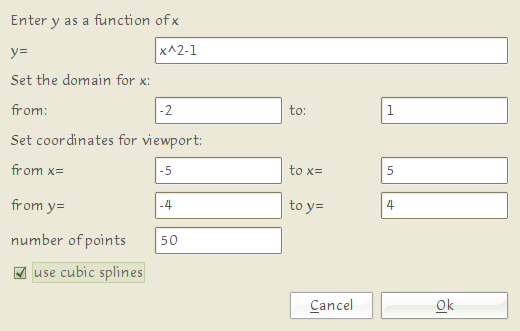
\includegraphics[scale=3]{secondline_dialog.png}
   \end{center}
   \caption{The dialog box for the second part of the plot of the piecewise
   function $f$}
   \label{fig:secondline_dialog}
\end{figure}

\begin{figure}[h]
   \begin{center}
      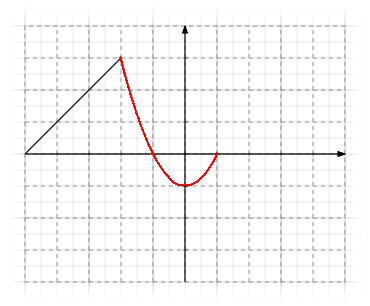
\includegraphics[scale=2]{secondline.png}
   \end{center}
   \caption{Plot of the first two parts of the piecewise function $f$}
   \label{fig:secondline}
\end{figure}

In a similar way, we create the third part of the plot.  Using \Ipe\ marks with
vertex snapping, you can place full and empty circles at the ends of the parts
of the graph to indicate whether the endpoints are included or not.  You can
also change the style of the plot curves to ``fat'' or ``ultrafat'' to make
them stand out against the coordinate grid.  The finished plot is at
Figure~\ref{fig:piecewise}. 

\begin{figure}[h]
   \begin{center}
      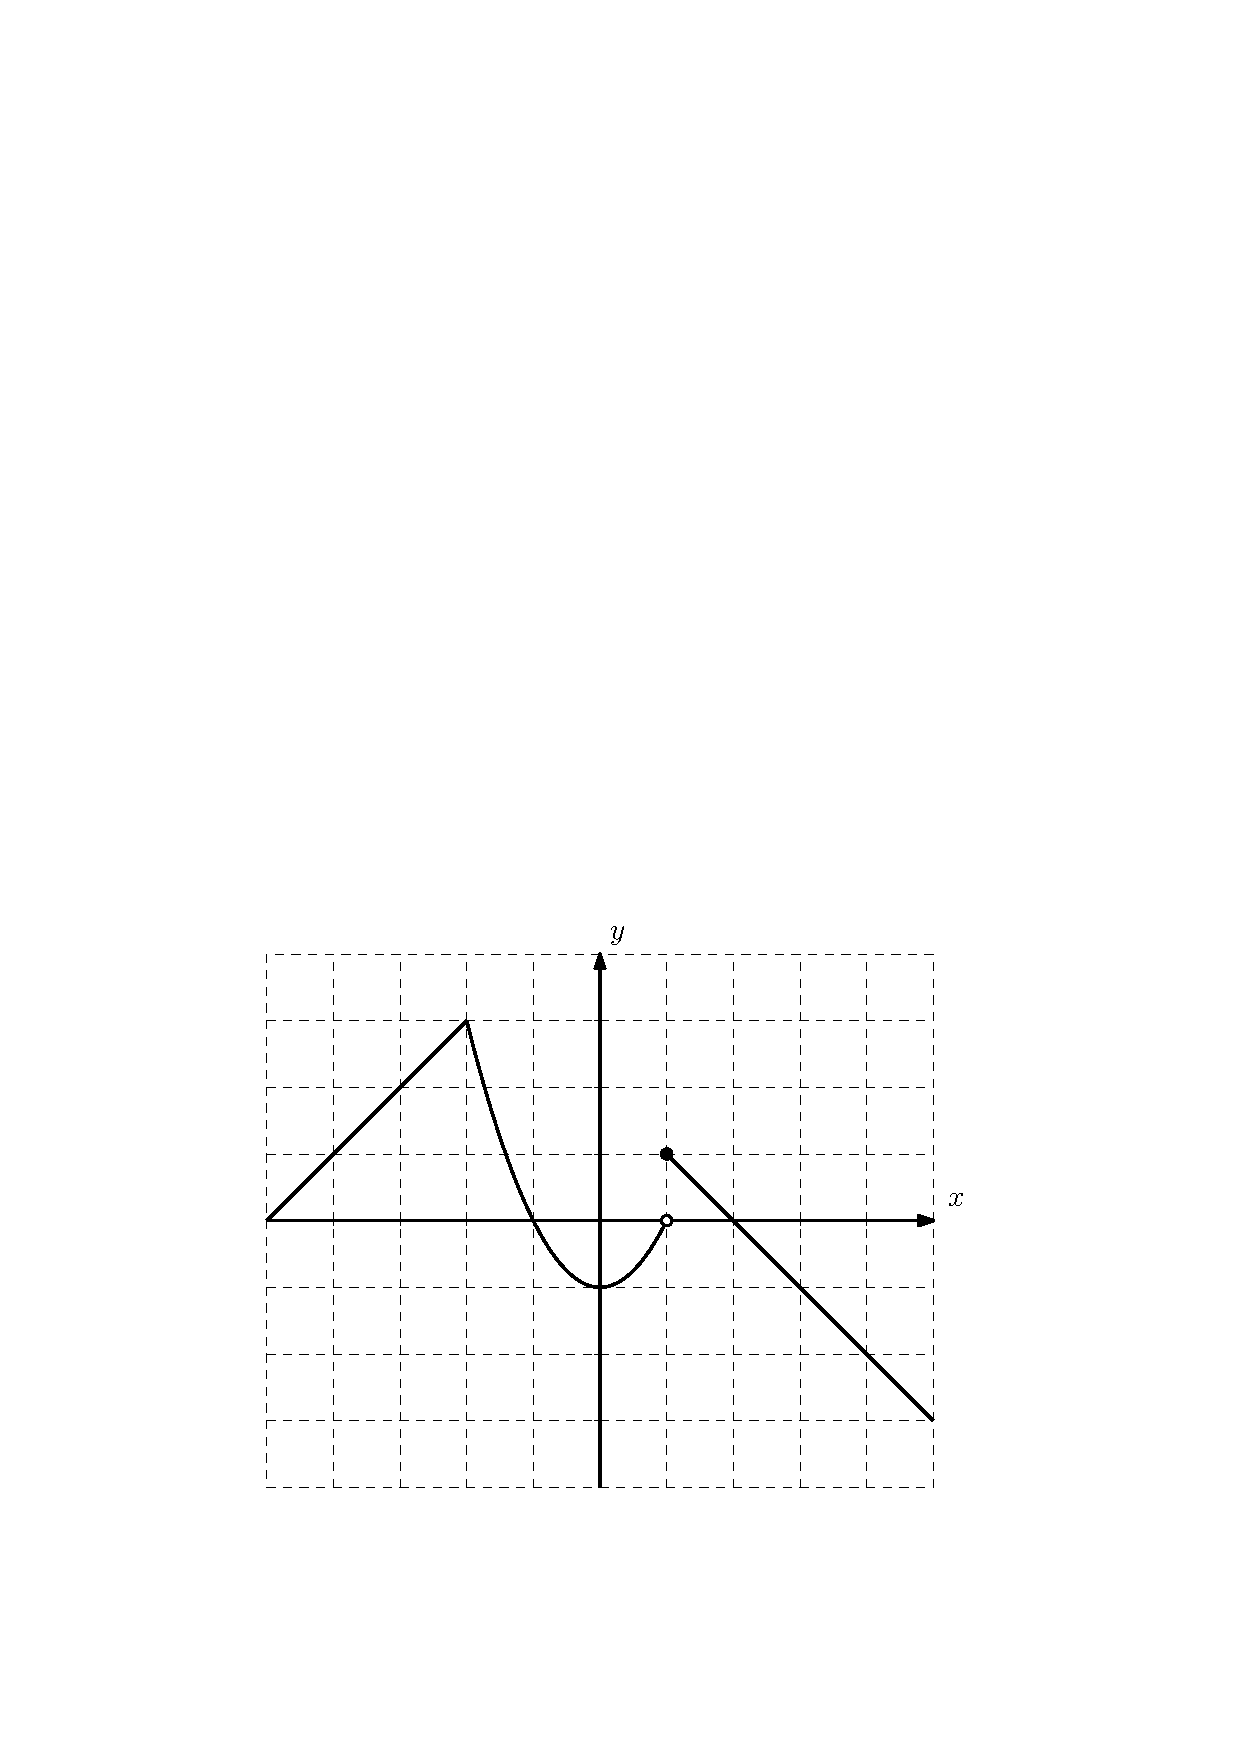
\includegraphics[scale=.7]{piecewise.pdf}
   \end{center}
   \caption{Graph of the piece wise function $f$}
   \label{fig:piecewise}
\end{figure}
\clearpage

\subsection{Function with Vertical Asymptote}\label{subsec:asymptote}

As the next example, we will plot the function 
\[g(x) = \frac{1}{1-x^2}.\]
The function is undefined at $\pm 1$ and has vertical asymptotes there. The
IpePlots ipelet is not smart enough to figure that out, and it will not be able
to plot the function properly.  It is our responsibility to choose the domain
of the plot properly.  We will plot the function for $x$ between $-4$ and $4$,
and $y$ between $-3$ and $3$.  Solving the equation 
\[\frac{1}{1-x^2} = -3\]
will give us $x = \pm \sqrt{4/3}$, solving the equation 
\[\frac{1}{1-x^2} = 3\]
results in $x = \pm \sqrt{2/3}$. 
We will plot the function on three intervals: $-4\le x \le -\sqrt{4/3}$,
$-\sqrt{2/3} \le x \le -\sqrt{2/3}$ and $\sqrt{4/3} \le x \le 4$. 
\begin{figure}[h]
   \begin{center}
      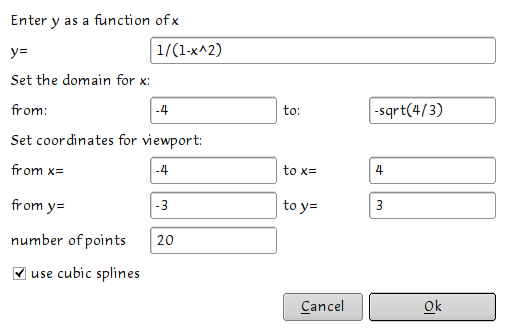
\includegraphics[scale=.5]{asym1.png}
   \end{center}
   \caption{The dialog to create the first part of the graph of $g$.}
   \label{fig:asym1}
\end{figure}

First we will create a coordinate system.  Then choose ``Function plot'' from
the ``Plots'' menu, and fill in the dialog as shown on Figure~\ref{fig:asym1}.
Note that it is possible to use expressions like \texttt{-sqrt(4/3)} in the
``from'' and ``to'' fields of the dialog.  Figure~\ref{fig:asym2} shows the
dialog for creation of the second part of the graph.  The third part can be
created in a similar way. Figure~\ref{fig:asym_plot} shows the resulting plot.

\begin{figure}[h]
   \begin{center}
      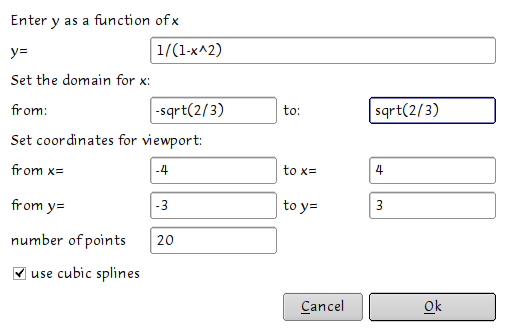
\includegraphics[scale=.5]{asym2.png}
   \end{center}
   \caption{The dialog to create the second part of the graph of $g$.}
   \label{fig:asym2}
\end{figure}
\begin{figure}[h]
   \begin{center}
      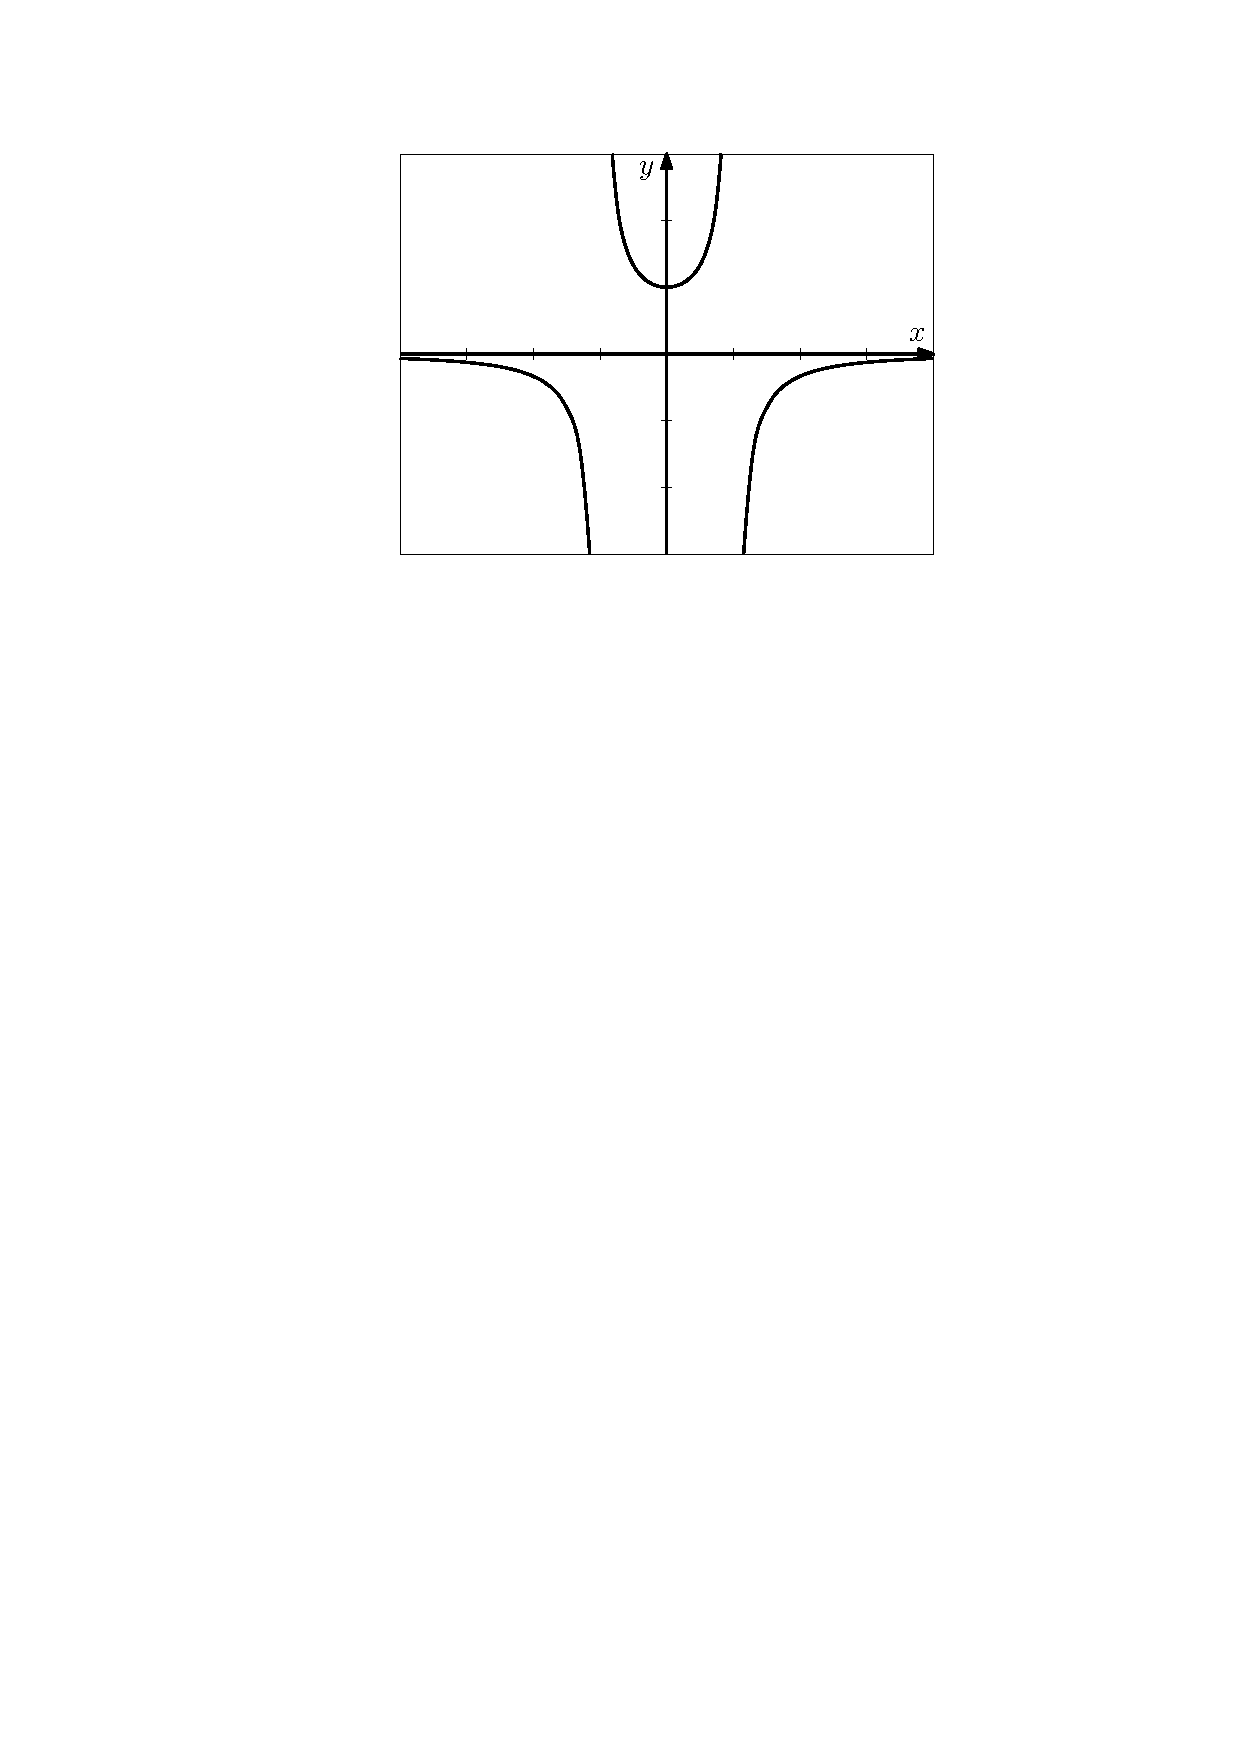
\includegraphics[scale=.7]{asym.pdf}
   \end{center}
   \caption{The final plot of the function $g$.}
   \label{fig:asym_plot}
\end{figure}
\clearpage

\subsection{Trigonometric Plot}
As a final example, we will plot a trigonometric function, with ticks on the
horizontal axis at multiples of $\pi/2$. We will start by creating a coordinate
system, for $x$ between $-2\pi$ and $2\pi$, and $y$ between $-2.2$ and $2.2$.
See Figure~\ref{fig:trig_coords}.  
\begin{figure}[h]
   \begin{center}
      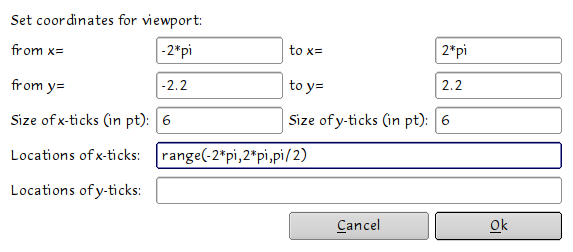
\includegraphics[scale=.5]{trig_coords.png}
   \end{center}
   \caption{The dialog to create the coordinate system for a trigonometric
   plot.}
   \label{fig:trig_coords}
\end{figure}
The most interesting part is the expression entered in the ``Location of
$x$-ticks'' field: \texttt{range(-2*pi,2*pi,pi/2)}. This will create ticks
uniformly distributed between $-2\pi$ and $2\pi$, with distance $\pi/2$ between
consecutive ticks.  

\begin{figure}[h]
   \begin{center}
      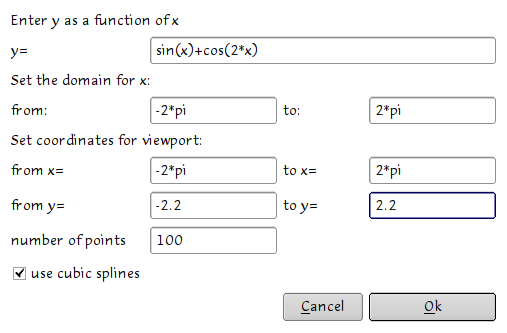
\includegraphics[scale=.5]{trig_dialog.png}
   \end{center}
   \caption{The dialog to create the coordinate system for a trigonometric
   plot.}
   \label{fig:trig_dialog}
\end{figure}
Next we will create the actual plot using the ``Function plot'' item from the
``Plots'' menu, as shown in Figure~\ref{fig:trig_dialog}. Finally, we change
the line thickness of the graph to ``ultrafat'', and add some legend to the
ticks on both horizontal and vertical axis. The resulting plot is shown in
Figure~\ref{fig:trig}

\begin{figure}[h]
   \begin{center}
      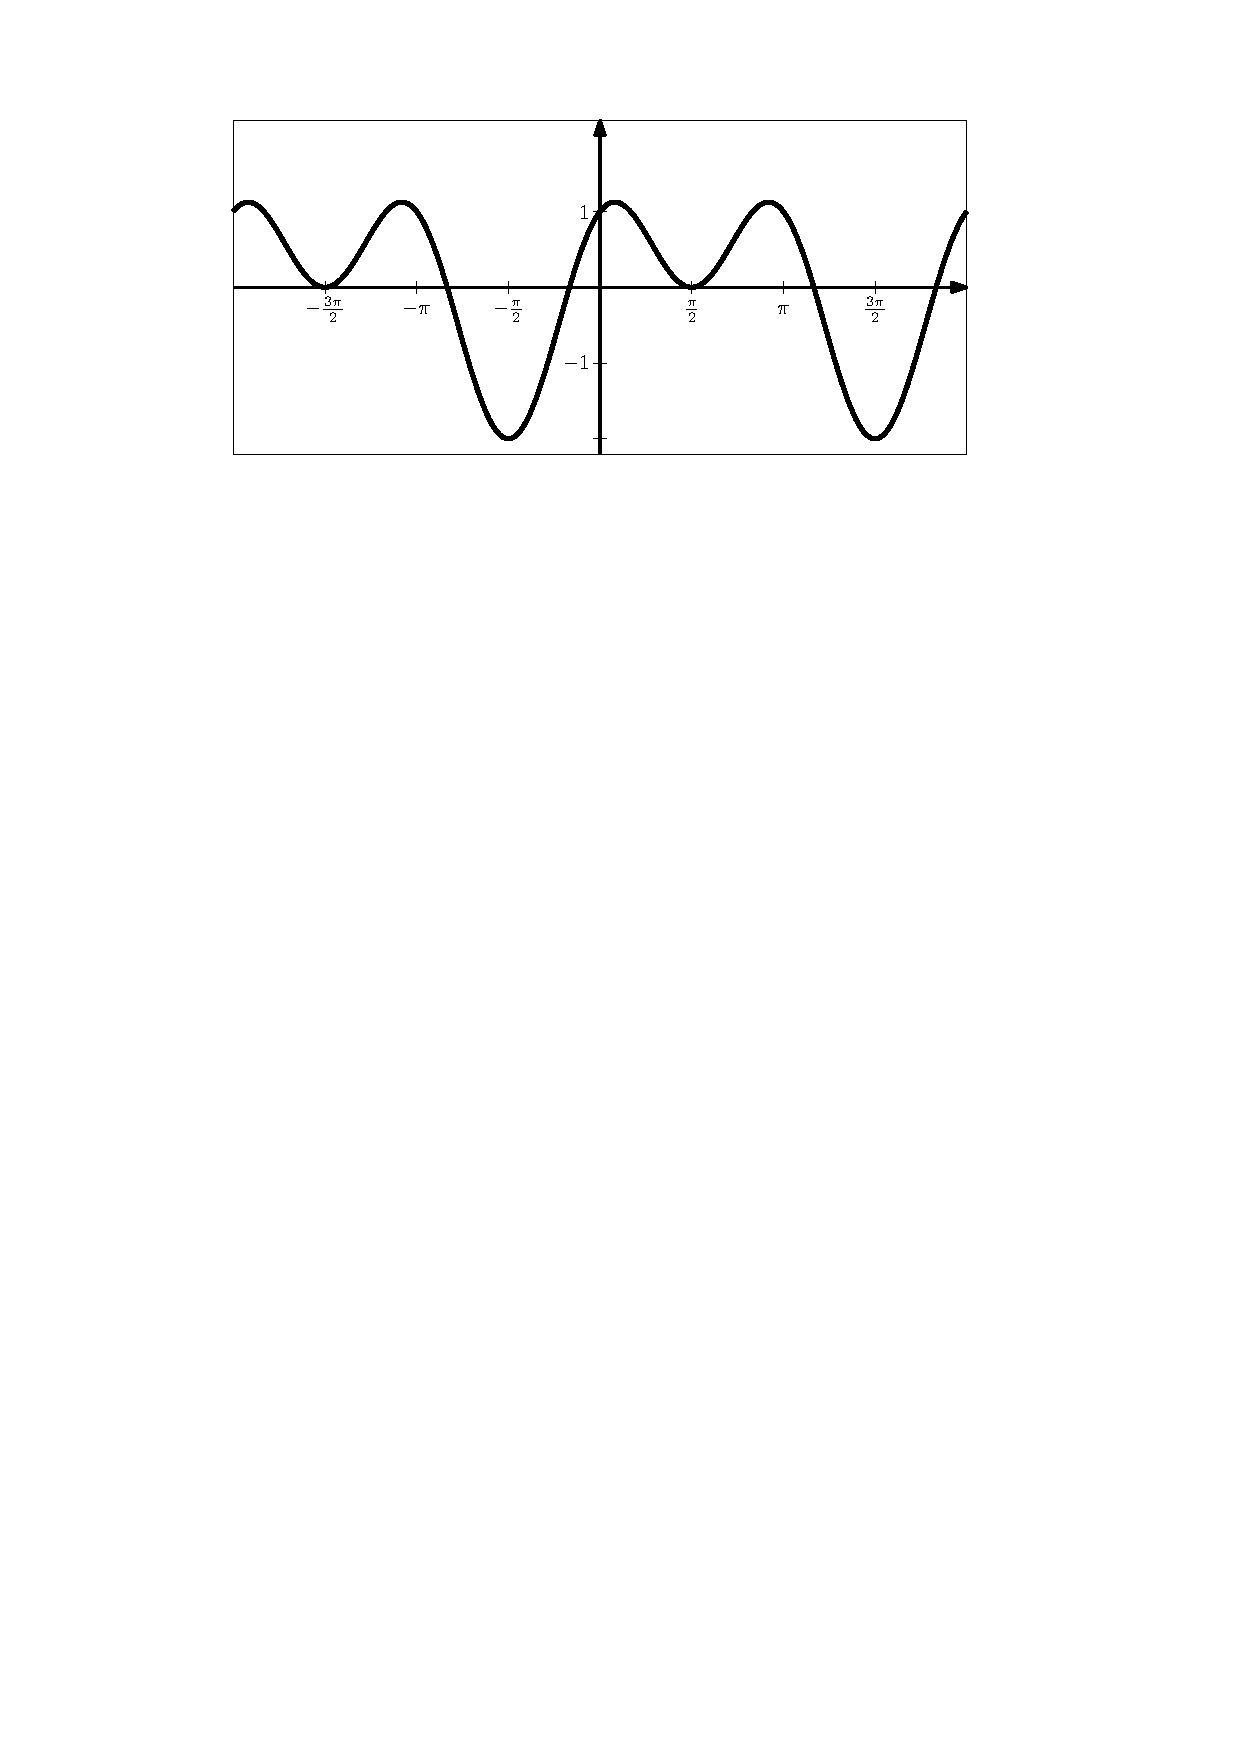
\includegraphics[scale=.7]{trig.pdf}
   \end{center}
   \caption{The final plot of the trigonometric function $\sin(x) + \cos(2x)$.}
   \label{fig:trig}
\end{figure}

\printbibliography
\end{document}
